\section{Umsetzung}
Hier noch generell was beschreiben. - Zielarchitekturbild darstellen (komplette Architektur)
Was wird im folgenden gemacht.

\colorbox{yellow}{Hier fehlt was}

\subsection{Cloud}
Hier beschreiben, was ich nun in der Cloud umsetzen will und warum man die Cloud eigentlich braucht. Vorteil der
Geschwindigkeit. Dabei würde es insgesamt vier Möglichkeiten geben das umzusetzen. Für welche habe ich mich
entschieden?

- Machine Learning Models (Autoamtisch aus Daten generrieren)\\
- Model flows (SPSS) - Make Deployment\\
- Model flows (SPSS) - Download Model - Import TensorFlow/TensorFlow.js\\
- Notebooks (Python)

\url{https://console.bluemix.net/docs/cli/index.html#overview}

\colorbox{yellow}{Hier fehlt was}

\subsubsection{Daten zusammenstellen}
\colorbox{yellow}{Hier fehlt was}

\subsubsection{Daten importieren}
Nachdem die Daten zusammengestellt sind, können diese nun in das Watson Studio importiert werden. Dazu gibt es im Watson
Studio einen Menüpunkt \texttt{Assets}. Dieser beinhaltet alle hochgeladenen, generrierten oder gesamelten Daten, Modelle,
Dashboards, Notebooks oder Flows. Die oberste Kategorie, \texttt{Data Assets}, beinhaltet alle Tabellen für die
Weiterverarbeitung.

In dieser kann über den Menüpunkt \texttt{New data asset} eine neue Datei hochgeladen werden. Ein klick auf diesen
Menüpunkt öffnet einen seitlichen Arbeitsbereich. In diesem kann über \texttt{browse} eine Datei ausgewählt werden.
Alternativ kann die Datei auch direkt in das farblich hervorgehobene Feld geschoben werden.

Im Anschluss sollte die Datei binnen weniger Sekunden hochgeladen sein und im Bereich Data assets angezeigt werden. Somit
ist der Upload fertiggestellt und die Datei kann umgewandelt werden.

\subsubsection{Daten umwandeln}
Da die erstellte Datei mit den Trainingssätzen nun in Watson Studio bereit steht, kann diese online in eine csv-Datei
umgewandelt werden. Dies ist zwingend notwendig, damit die Datei später als Eingabeparameter für das neuronale Netz dienen
kann. Ein anderes Format wird zur Zeit nicht unterstützt.

In Watson Studio liegt mit den \texttt{Data flows} ein einfaches Werkzeug bereit, um Dateien in das benötigte csv-Format
zu überführen. Dazu wird in der Kategorie Data flows über \texttt{New data flow} ein neuer Flow angelegt.

Im folgenden öffnet sich der Wizzard zum Erstellen des Flows. Als erster Schritt muss im linken Bereich die Datei
ausgewählt werden, welche konvertiert werden soll. Über \texttt{Add} kann die Auswahl übernommen werden.

Nun wird der Inhalt der Datei angezeigt. Es ist darauf zu achten, dass die Werte der einzelnen Spalten als Dezimal-Zahl
interpretiert werden. Falls dies nicht Voreingestellt ist, kann das in jede Spalte über die drei Punkte (Einstellungen)
und den Eintrag \texttt{Convert Column} getätigt werden. Der Wert sollte dann auf \texttt{Decimal} gestellt werden.

Nachdem nun alle Einträge als Dezimal-Zahl interpretiert werden, kann die Konvertierung über \texttt{Run data flow}
gestartet werden. Zum Abschluss wird noch eine Übersicht über die einzelnen Schritte gegeben, die zur Konvertierung
notwendig sind. Hier werden zum Beispiel etwaige Konvertierungen zu Dezimal-Zahlen angezeigt oder sonstige Operationen
dargestellt. Die Seite kann bestätigt werden und der Flow sollte starten.

Nach wenigen Minuten sollte im Watson Studio im Bereich Assets, in der Kategorie Data assets, die neue Datei zur Verfügung
stehen. Dabei trägt die Datei die Dateiendung csv. Die Konvertiedung der Datei ist somit abgeschlossen und sie kann für
das neuronale Netz verwendet werden.

\subsubsection{Modeler flow}
Nach erfolgreicher Konvertierung der Trainingsdaten, können diese für das neuronale Netz genutzt werden. Für die
Erstellung des neuronalen Netzes und den damit verbundenen Parameterübergaben wird \texttt{Modeler flow} genutzt.

Im Bereich Assets kann dieser über die Schaltfläche \texttt{New flow} erstellt und eingerichtet werden. Nach der definition
des Namens für den Flow und einer optionalen Beschreibung, sollte \texttt{Modeler flow} und \texttt{IBM SPSS Modeler}
ausgewählt werden. Nachdem die richtigen Punkte ausgewählt wurden, kann der Modeler flow über \texttt{Create} erstellt
werden. Nach kurzer Zeit wird ein leerer Arbeitsbereich für das Erstellen des Flows angezeigt.

Über den Menüpunkt \texttt{Palette} kann ein linker Arbeitsbereich angezeigt werden, welcher alle Module, die genutzt
werden können, gruppiert anzeigt. Damit die konvertierten Trainingsdaten vom neuronalen Netz genutzt werden können,
müssen sie über den Baustein \texttt{Data asset} in der Gruppe Import eingebaut werden. Das Modul kann über Drag\&Drop
auf dem leeren Arbeitsbereich positioniert werden.

Im Anschluss muss das Modul konfiguriert werden. Der Konfigurator kann über ein doppelten Klick auf das entsprechende
Modul angezeigt werden. Die Einstellungen öffnen sich am rechten Seitenrand. Nun muss über den Knopf
\texttt{Change Data Asset} die konvertierte Datei ausgewählt werden. Mit einem Klick auf Save werden die Informationen
gespeichert.

Als nächstes muss das neuronale Netz eingebaut werden. In der Kategorie \texttt{Modeling} gibt es das Modul
\texttt{Neural Net} welches für die Anwendung die beste Alternative darstellt. Auch dies kann mit der Maus in einen
freien Bereich des Arbeitsbereiches geschoben werden.

Damit die Daten, welche durch das Import-Modul geladen, auch im neuronalen Netz genutzt werden können, muss eine
Verbindung zwischen Import und neuronalem Netz gezogen werden. Dies kann durch einen Klick auch den Ausgang des
Data Assets gestartet werden. Im Anschluss muss noch der Eingang des neuronalen Netz angeklickt werden. Nun besteht eine
Verbindung zwischen den beiden Modulen.

Bei einer Verbindung werden die Ausgaben des jeweiligen Modules weiter an die mit einer Linie verbundenen Module
weitergegeben. Diese Folgemodule können die Werte dann als Eingabevariablen nutzen.

Das hinzugefügte neuronale Netz Modul kann durch einen doppelten Klick konfiguriert werden. Auf der rechten Seite muss
der Hacken bei \enquote{Use custom field roles} gesetzt werden. Diese Einstellung sorgt dafür, dass die \texttt{Targets}
und die \texttt{Inputs} manuell konfiguriert werden können.

Die Tabelle \ref{tab:targets_inputs} auf Seite \pageref{tab:targets_inputs} gibt einen Überblick über die Auszuwählenden
Variablen in den beiden Feldern \texttt{Targets} und \texttt{Inputs}. Dabei beschreiben die Targets die Variablen, welche
durch den Watson Service Vorhergesagt werden sollen. Die Inputs definieren die Größen, durch welche eine Vorhersage
überhaupt möglich ist.

Das Model wird zu einem späteren Zeitpunkt mit den \textit{Inputs} gefüttert und die \textit{Targets} kommen als
vorhergesagte Rückgabeparameter zurück.

\begin{table}[hb]
    \centering
    \begin{tabular}{|c|c|}
        \hline
        \textbf{Targets} & \textbf{Inputs}\\
        \hline
        \hline
        Druckluft & Einlaufbandlänge\\
        \hline
        Impuls & Wägebandlänge\\
        \hline
        Totzeit & Auslaufbandlänge\\
        \hline
        Position & Einlaufbandbreite\\
        \hline
         & Wägebandbreite\\
        \hline
        & Auslaufbandbreite\\
        \hline
        & Einlaufbandrolle\\
        \hline
        & Wägebandrolle\\
        \hline
        & Auslaufbandrolle\\
        \hline
        & Produktbreite\\
        \hline
        & Produktlänge\\
        \hline
        & Produkthöhe\\
        \hline
        & Leistung\\
        \hline
        & Packungsgewicht\\
        \hline
    \end{tabular}
    \caption{Variablen für die Targets und Inputs}
    \label{tab:targets_inputs}
\end{table}

Alle anderen Parameter für das neuronale Netz können in der ersten Version erst Mal auf Standardeinsellungen belassen
werden. Zu einem späteren Zeitpunkt, bei wechselnden Testdaten, können diese verändert werden um die Vorhersagen
genauer zu machen.

Der Flow für das neuronale Netz ist fertiggestellt und kann gestartet werden. Dadruch wird das neuronale Netz trainiert
und das fertige Model erscheint in der Übersicht. Dies kann durch ein Klick auf den \texttt{Run} Button getätigt werden.

Nach ein paar Minuten wird unterhalb des neuronalen Netz Moduls ein weiteres Modul angezeigt. Dabei handelt es sich um
das trainierte neuronale Netz. Dies wird auch durch eine gestrichelte Linie symbolisiert, welche sich zwischen dem
eigentlichen neuronalen Netz und dem trainierten Model befindet, visualisiert.

Damit das trainierte Model in einem weiteren Schritt in einem deployment verfügbar gemacht werden kann, muss es die
Möglichkeit der Exportierung geben. Aktuell ist es nicht möglich, dieses über ein Kontextmenü zu tätigen. Für den Export
wird ein weiteres Modul benötigt, die \texttt{Table}.

Das Table-Modul befindet sich in der Kategorie \texttt{Outputs} und kann, genau wie alle andere Module, frei auf dem
Arbeitsbereich platziert werden. Anschließend muss es mit der Ausgabe des trainierten Models verbunden werden. Es ist
keine Konfiguration des Models notwendig.

Nach der erfolgreichen Verbindung, kann die Table mit der rechten Maustatse angeklickt werden. Im Kontextmenü kann über
\enquote{Save branch as a model} das neue Model erstellt werden. Nach der Eingabe eines Namens, wird das Model erstellt
und ist im Watson Studio Dashboard in der Kategorie Assets sichtbar.

In Abbildung \ref{fig:umsetzung_model_flow} auf Seite \pageref{fig:umsetzung_model_flow} ist der vollständige Aufbau des
Model flows visualisiert.

\begin{figure}[h]
    \centering
    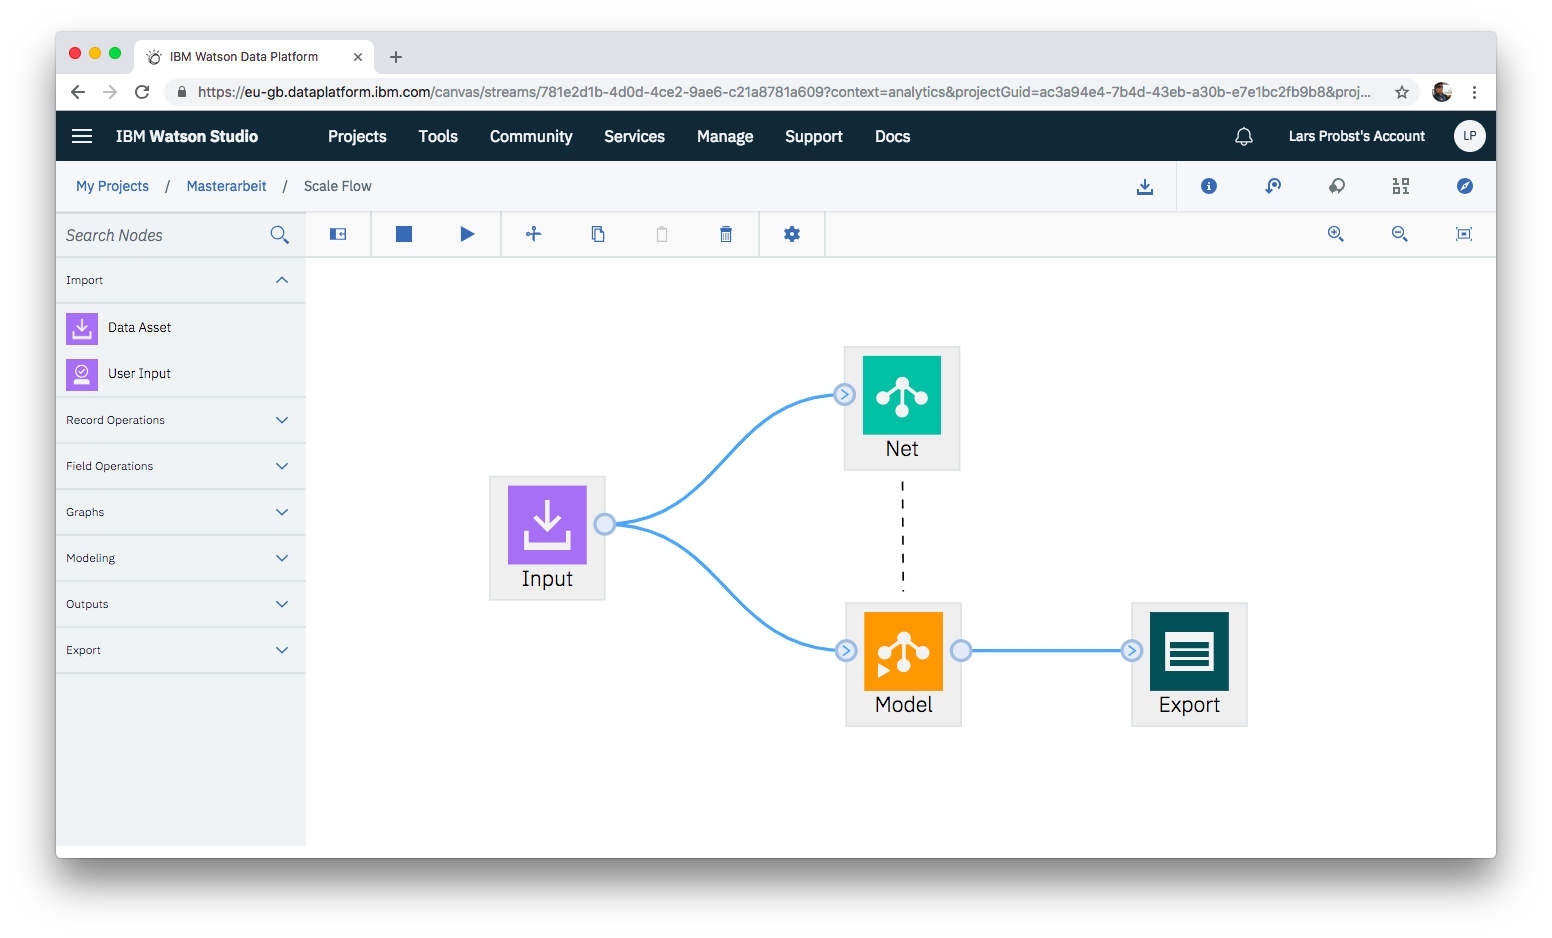
\includegraphics[scale=0.26]{images/kapitel_3/umsetzung_model_flow.png}
    \caption{Kompletter Model flow}
    \label{fig:umsetzung_model_flow}
\end{figure}

\subsubsection{Informationen zum Model}
\colorbox{yellow}{Beschreiben von den ganzen Informationen von dem Model. Rechte Maustaste - View}

\subsubsection{Deployment erstellen}
Das im vorangegangenen Kapitel erstellte und trainierte Model kann im weiteren durch ein Deployment über eine
REST-Schnittstelle verfügbar gemacht werden. Dazu ist es erforderlich, das Model in einen \texttt{Web service} zu
installieren. Die spätere Wartung und Verwaltung wird dabei von Bluemix übernommen.

Damit der Web Service erstellt werden kann, muss im Watson Dashboard das Model ausgewählt werden. Das folgende Fenster
zeigt mehrere Informationen zu diesem. Unter anderem ist sichtbar, welche Eingabe- und Ausgabeparameter für das Model
wichtig sind.

Über den Reiter \texttt{Evaluation} können vorangeganene Auswertungen angezeigt werden und der Menüpunkt \texttt{Lineage}
zeigt die Verknüpfungen und Abstammungen des Models an.

Für das Deployment ist der Reiter \texttt{Deployments} wichtig. Über diesen können alte Deployments gelöscht oder neue
hinzugefügt werden. Über den oben rechts befindlichen Link \texttt{Add Deployment} wird ein solches neu hinzugefügt. Als
Name kann hier ein beliebiger vergeben werden. Als \texttt{Type} sollte Web Service ausgewählt sein. Ein klick auf
\texttt{Save} speichert die Einstellungen und erstellt das Deployment. Dieser Vorgang kann bis zu zenh Minuten dauern.

Im Anschluss wird in der Spalte \textit{Status} der Wert \texttt{DEPLOY\_SUCCESS} angezeigt. Damit ist das Deployment
erfolgreich abgeschlossen. Mit einem klick auf den eingerichteten Namen des Deployments öffnet sich eine
Informationsseite.

\subsubsection{Deployment testen}
Das freigegebene Deployment kann nun über das Watson Studio Dashboard online getestet werden. Dies hat den Vorteil, dass
das Deployment direkt getestet werden kann um das Model zu überprüfen.

Über den Menüpunkt \textit{Deployments} im eingerichteten Model kann über den Link im Namen das Deployment angeschaut
werden. Hier stehen neben diversen Informationen auch der Menüpunkt \texttt{Test} zur Verfügung. In diesem öffnet sich
eine zweispaltige Ansicht auf der im linken Bereich die Eingabefelder befüllt werden können. Nach erfolgreicher Eingabe
kann über den Button \texttt{Predict} eine Vorhersage gestartet werden.

Nach wenigen Sekunden erscheint auf der rechten Seite ein langes JSON-Object, welches den Rückgabewert des Web Services
aufzeigt. Das erste Array, \texttt{fields}, listet die Felder auf, welche an den Web-Service gesendet wurden.

Das zweite Array, \texttt{values}, zeigt anfangs die Werte, welche an den Web Service gesendet wurden. Die letzten fünf
Werte entsprechen den Vorhersagen des trainierten Models.

Sollte das Array \textit{values} kleiner sein als das Array \textit{fields}, war das trainieren des Models nicht
erfolgreich.

\subsubsection{Aufruf mit Postman}
\label{subsec:Aufruf mit Postman}
Im Weiteren soll das erstellte Model, welches über ein Deployment in einem Web-Service zur Verfügung gestellt wurde,
mit Postman\footnote{https://www.getpostman.com} getestet werden.

So ist sichergestellt, dass das Model auch von extern, nicht nur über das Watson Studio Dashboard, aufrufbar ist.
Dies ist für die spätere Entwicklung des Frontends und die Einrichtung des API Connect Services wichtig. Außerdem können
so die Übergabeparameter und die Rückgabewerte der Schnittstelle überprüft werden.

Um auf die Schnittstelle des Web-Services zugreifen zu können, muss bei jedem Request an diesen ein
\textit{Authentication Token} (kurz Auth-Token) mitgeschickt werden. Dieser Token stellt sicher, dass es sich um einen
gültigen Aufruf handelt.

Der Token kann über eine REST-Schnittstelle des Watson Studio erstellt werden. Dabei handelt es sich um eine andere
Schnittstelle als beim Web-Service. Der Token ist immer nur für maximal vier Stunden gültig.

Um einen Auth-Token zu erstellen, muss der Watson Studio Benutzername und das zugehörige Passwort an die Schnittstelle
übergeben werden. Ein Beispielaufruf ist in Listing~\ref{Abruf des Auth-Tokens} auf Seite~\pageref{Abruf des Auth-Tokens}
zu sehen. Der Token ist dabei in einem JSON-Object im Rückgabewert.

\begin{lstlisting}[language=bash, caption=Abruf des Auth-Tokens, label=Abruf des Auth-Tokens]
$ curl --basic --user USERNAME:PASSWORD https://eu-gb.ml.cloud.ibm.com/v3/identity/token
\end{lstlisting}

In Postman kann dieser Aufruf durch die Eingabe der URL und dem HTTP-Type \texttt{GET} gemacht werden. Im Reiter
\texttt{Authentication} muss als Type \texttt{Basic-Auth} ausgewählt werden.

Im rechten Bereich sollten dann die beiden Eingabefelder für Benutzername und Passwort erscheinen. Nach der Eingabe der
geforderten Daten kann mit \texttt{Send} der Request abgeschickt werden und nach wenigen Sekunden sollte der Token in
einem JSON-Object als Rückgabeparameter erscheinen.

Anschließend kann ein neuer Postman-Tab geäffnet werden, welcher das eigentliche Deployment aufrufen soll. Der
REST-Endpunkt ist in Watson Studio unter Deployments zu finden und heißt \texttt{Scoring End-point}.

Dieser Scoring End-point kann als URL in Postman eingetragen und als HTTP-Type muss \texttt{POST} ausgewählt werden. Im
Bereich \texttt{Authentication} wird der Type mit \texttt{Baerer} angegeben. Somit kann im rechten Bereich nicht der
Benutzername und das Passwort angegeben werden, sondern gespeicherte Token.

Durch die Auswahl des HTTP-Types \textit{POST} kann der \texttt{Body} des Requests definiert werden. Dabei handelt es
sich um Parameter, welche an die Schnittstelle mitgeschickt werden. Für das Deployment ist es wichtig, dass die Daten
in Postman als \texttt{raw} und Type \texttt{JSON (application/json)} geschickt werden. Nun können in das Feld eigene
Testparameter eingetragen werden. Im Anhang \ref{sec:postmanTestparameter} auf Seite \pageref{sec:postmanTestparameter}
findet sich dafür ein Beispiel.

Abschließend kann mit Button \texttt{Send} der Request abgeschickt werden. Nach wenigen Sekunden erhält man den Response
des neuronalen Netzes als Rückgabeparameter angezeigt. Hier sollten auch die Vorhersagen enthalten sein.

Auf der Übersichtsseite des REST-Interfaces des
Deployments\footnote{https://watson\-ml\-api.mybluemix.net/?cm\_mc\_uid=61889453441915363064337}, können noch weitere
Endpunkte und die dafür benötigten Parameter sowie die Rückgabewerte eingesehen werden.

\subsection{TensorFlow.js}
Da die Watson Studio Applikation nun erfolgreich in einem Deployment zur Verfügung gestellt und der Aufruf über
Postman verifiziert wurde, kann nun das trainierte Model in eine TensorFlow.js Applikation eingebettet werden.

Einrichten der Node.js-Umgebung auf dem PC. Dann entwicklen des ganzen. Dazu muss das trainierte Netz, welches im
vorangegangenen Kapitel erstellt wurde heruntergeladen werden. Dann in TensorFlow.js einbinden und nutzen. Also einen
Wrapper bauen. Gerade interessant für On The Edge Sachen oder für Mobile.

\colorbox{yellow}{Hier fehlt was}

\subsubsection{Model Exportieren}
\colorbox{yellow}{Hier fehlt was}

Damit die Applikation über eine Domain aus dem Internet aus aufrufbar ist, muss diese zum Beispiel in einen Cloud
Foundry-Container, welcher in der IBM Cloud läuft, installiert werden. Im folgenden Kapitel werden die dafür nötigen
Schritte erläutert.

\subsection{Toolchain einrichten}
Da die Node.js-Applikation fertig entwickelt ist, soll diese in einem Cloud Foundry-Container installiert und über eine
Domain abrufbar gemach werden. Damit dies nicht manuell nach jeder Änderung im Quellcode über \texttt{cf push} gemacht
werden muss, kann eine Toolchain aus der IBM Cloud genutzt werden.

Für die Nutzung der Toolchain wird ein Git-Repository angelegt. Nach jedem \texttt{commit}, welcher in dieses Repository
geschrieben wird, aktiviert sich die Toolchain selbstständig und lädt den entsprechenden Commit herunter.

Anschließend werden, je nach gewählter und eingerichteter Konfiguration, verschiedene Schritte (Phasen) in der Toolchain
durchlaufen, um die Applikation in einen Cloud Foundry-Container zu installieren.

Dabei können die einzelnen Schritte, welche beim Deployment durchlaufen werden, selbst definiert, oder eine
vorkonfigurierte Toolchain genutzt werden. Die vorkonfigurierte Toolchain kann im Nachgang allerdings individuell
angepasst werden und dient lediglich einem schnelleren Start.

Für die Konfiguration der Toolchain muss die instanziierte Node.js-Runtime, in welcher die entwickelte Applikation laufen
soll, in dem IBM Cloud Dashboard ausgewählt werden.

Auf der folgenden Seite, im Tab \texttt{Übersicht} (linke Seite), erscheinen fünf Kacheln mit unterschiedlichen Informationen.
Für die Toolchain ist die Karte mit der Aufschritf \texttt{Continous Delivery} entscheidend. Dort gibt es einen Button
mit der Aufschrift \texttt{Aktivieren}.

Ein Klick auf diesen öffnet die Übersicht und eine visuelle Vorschau der Standardkonfiguration der Toolchain. Nun kann ein
Name eingetragen und die Region ausgewählt werden, in der die Toolchain installiert werden soll. Da die Standardkonfiguration
vorerst völlig ausreichend ist, kann diese direkt übernommen werden. Dafür genügt ein Klick auf \texttt{Erstellen}.

Nach einem kurzen Ladevorgang wurde die Toolchain eingerichtet und vorkonfiguriert. Es erscheinen nun vier Karten für
unterschiedliche Bereiche, in denen die IBM Cloud dem Entwicklungszyklus helfen kann.

Im Bereich \texttt{Nachdenken} wird ein Issue-Tracker konfiguriert, in dem zum Beispiel Bugs (Softwarefehler), welche
in der Software entdeckt werden, eingetragen, verwaltet und diskutiert werden können.

In \texttt{Codieren} stehen gleich zwei Kacheln zur Verfügung. Einerseits das konfigurierte Git-Repository, bei dem es
sich um ein auf IBM-Servern gehostetet GitLab handelt. Andererseits findet sich dort eine Web-IDE, auf Basis von Eclipse
Orion, mit der der Quellcode der Anwendung online editiert werden kann.

Im der letzten Kategorie, \texttt{Bereitstellen}, findet sich die Pipeline, welche im nächsten Schritt näher Erläutert
und eingerichtet wird. Ein Klick auf die Kachel mit der Aufschrift \texttt{Delivery Pipeline} öffnet diese.

Nach dem Laden der Seite erscheinen zwei sogenannte \texttt{Phasen} (engl. Stages). Jeder Schritt in der Delivery Pipeline
wird durch eine Phase symbolisiert. In einer Phase können zum Beispiel der Quellcode aus dem Git-Repository geladen, oder
die geschriebenen Tests durchgeführt werden.

Die Standardkonfiguration sieht in der \texttt{Build Stage} das Herunterladen des Quellcodes aus dem Git-Repository vor
und in der \texttt{Deploy Stage} das Einrichten eines Cloud Foundy-Containers.

Für die Node.js-Applikation reicht diese Konfiguration völlig aus, da keine zusätzlichen Installationen oder Einrichtungen
notwendig sind.

Als nächstes muss der geschriebene Quellcode der Applikation lediglich noch in das, in der Toolchain hinzugefügte,
Git-Repository eingecheckt werden. Die URL für das Repository kann in der Toolchain-Übersicht mit einem Klick auf die
Kachel \texttt{Git} angezeigt werden.

Nach erfolgreichem \texttt{push} der Anwendung in das Git-Repository startet der deployment Vorgang in der Toolchain
selbstständig. Nach wenigen Minuten sollte die Anwendung über ihre URL, welche in der Node.js Runtime definiert ist,
aufrufbar sein.

Da die Applikation nun im Internet in einem Cloud Foundry-Container zur Verfügung steht, kann diese im nächsten Schritt
mit dem API Connect Service verbunden werden. Dieser Schritt ist nötig, damit die Schnittstelle der Applikation vom
Frontend, welches in Kapitel~\ref{subsec:webseite} auf Seite~\pageref{subsec:webseite} beschrieben wird, und über Postman
vereinfacht aufgerufen werden kann.

\subsection{API Connect}
Wie in Kapitel \ref{subsec:Aufruf mit Postman} auf Seite \pageref{subsec:Aufruf mit Postman} beschrieben, benötigt das
REST-Interface des erstellten Deployments einen Auth-Token. Dieser kann nur über den Aufruf einer anderen
REST-Schnittstelle zur Verfügung gestellt werden.

Damit dies vereinfacht werden und das im weiteren Verlauf erstellte Frontend ebenfalls das Deployment aufrufen kann,
werden beide Abfragen in API Connect gebündelt.

Ein weiterer Grund für das Bündeln der beiden Anfragen an den Watson Service ist das mitschicken des Benutzernamens und
des zugehörigen Passwortes zum generrieren des Tokens. Damit diese nicht in der zu entwickelnden Anwendung hinterlegt
werden müssen, können diese Zentral in API-Connect gespeichert werden.

Das hat den Vorteil, dass sie bei Bedarf nur an einer Stelle abgeändert werden müssen. Auch werden sie nicht in einer
Anwendung hinterlegt, in der sie relativ einfach abgefangen und zu anderen Zwecken genutzt werden können.

Ein weiterer Vorteil für die Nutzung von API Connect ist die Tatsache, dass es zwei Möglichkeiten gibt, Vorhersagen zu
beziehen. Nebem dem Deployment des Watson Models kann auch die Schnittstelle der Node.js-Applikation mit TensorFlow.js
genutzt werden.

Mittels API Connect können Aufrufe optimal verteilt und Änderungen können schnell und komfortabel mit einem Online-Editor
angepasst werden.

\subsubsection{API Connect einrichten}
Da der Service, wie in Kapitel \ref{subsec:apiconnect} auf Seite \pageref{subsec:apiconnect} beschrieben, schon
eingerichtet wurde, kann dieser nun über IBM Bluemix Dashboard aufgerufen werden.

\colorbox{yellow}{Hier fehlt was}